\documentclass{cernrep}
\begin{document}
\title{PF hadron calibration}
\author{Changgi Huh}
\institute{Kyungpook National University, Republic of Korea}

\maketitle

Code description of PF hadron calibration.
Running with "root calibChris.C"

\section{functions}

The main function of this code is calibChris(). Inside of calibChris(), some functions and classes are used. The function list is 
\begin{itemize}
\item InitBarrelAlpha()
\item LoadOldThresholds()
\item getValuesFromTree(vector<double>\&, vector<double>\&, vector<double>\&, vector<double>\&, vector<double>\&)
\item GetETrueBin(double)
\item GetETrueBinEta(double)
\item assignvalues(vector<float>*, vector<float>*, vector<float>*, vector<float>*)
\item drawCompare(TGraph\&, TGraph\&, TGraph\&, TGraph\&)
\item drawEtaDependence(TH2F*, TGraph*)
\item drawGausFit(TH2F*, TGraph*, TGraph*, TString)
\end{itemize}

The class list is

\begin{itemize}
\item ABC
\item AlphaBeta
\end{itemize}

Inside of two classes, several functions are exist. The lists are in the Figure \ref{ABC} and Figure \ref{AlphaBeta}. Detail descriptions are written in below.

\begin{figure}[ht]
%\begin{center}
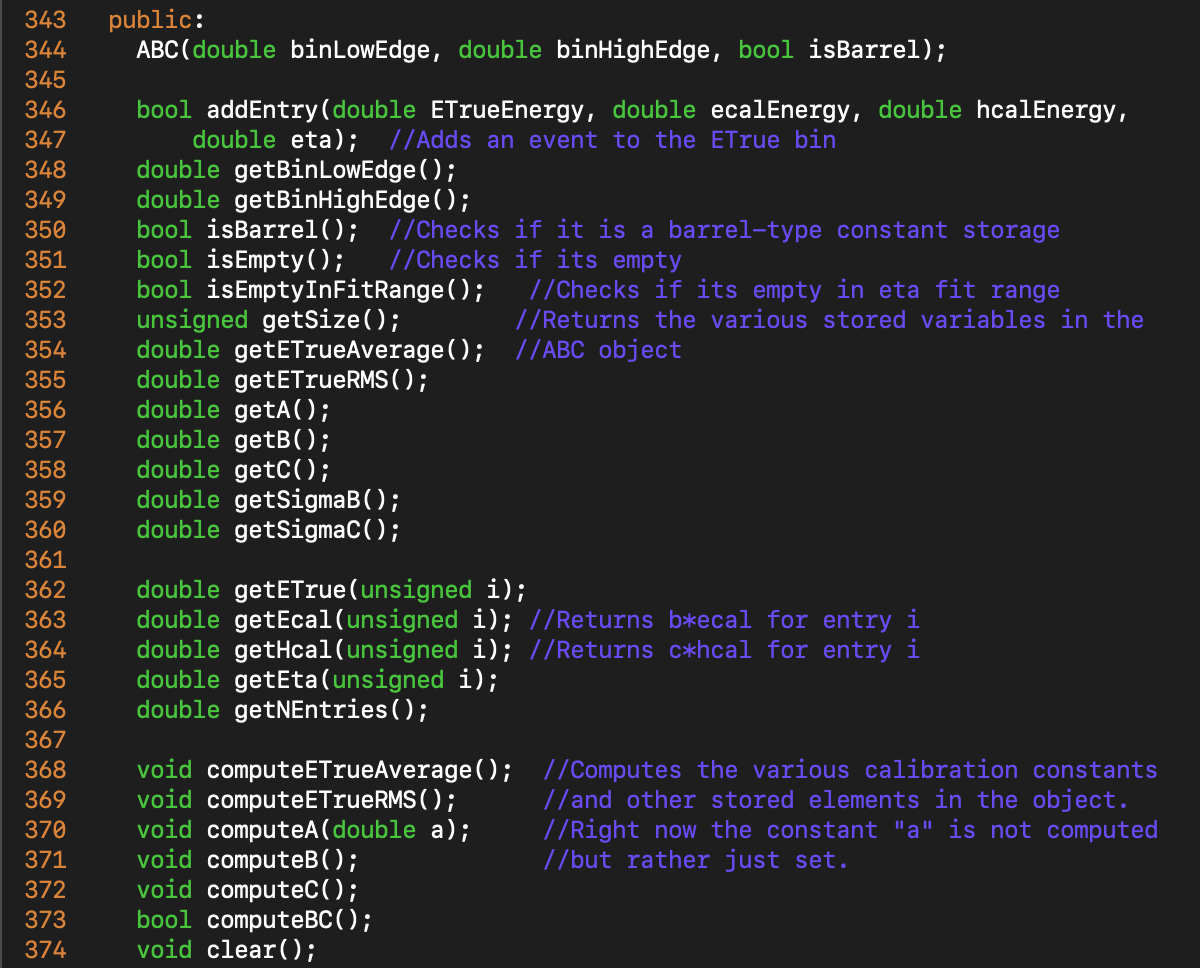
\includegraphics[width=1.0\textwidth]{fig/ABC.png}
\caption{functions in ABC class}
\label{ABC}
%\end{center}
\end{figure}

\begin{figure}[ht]
%\begin{center}
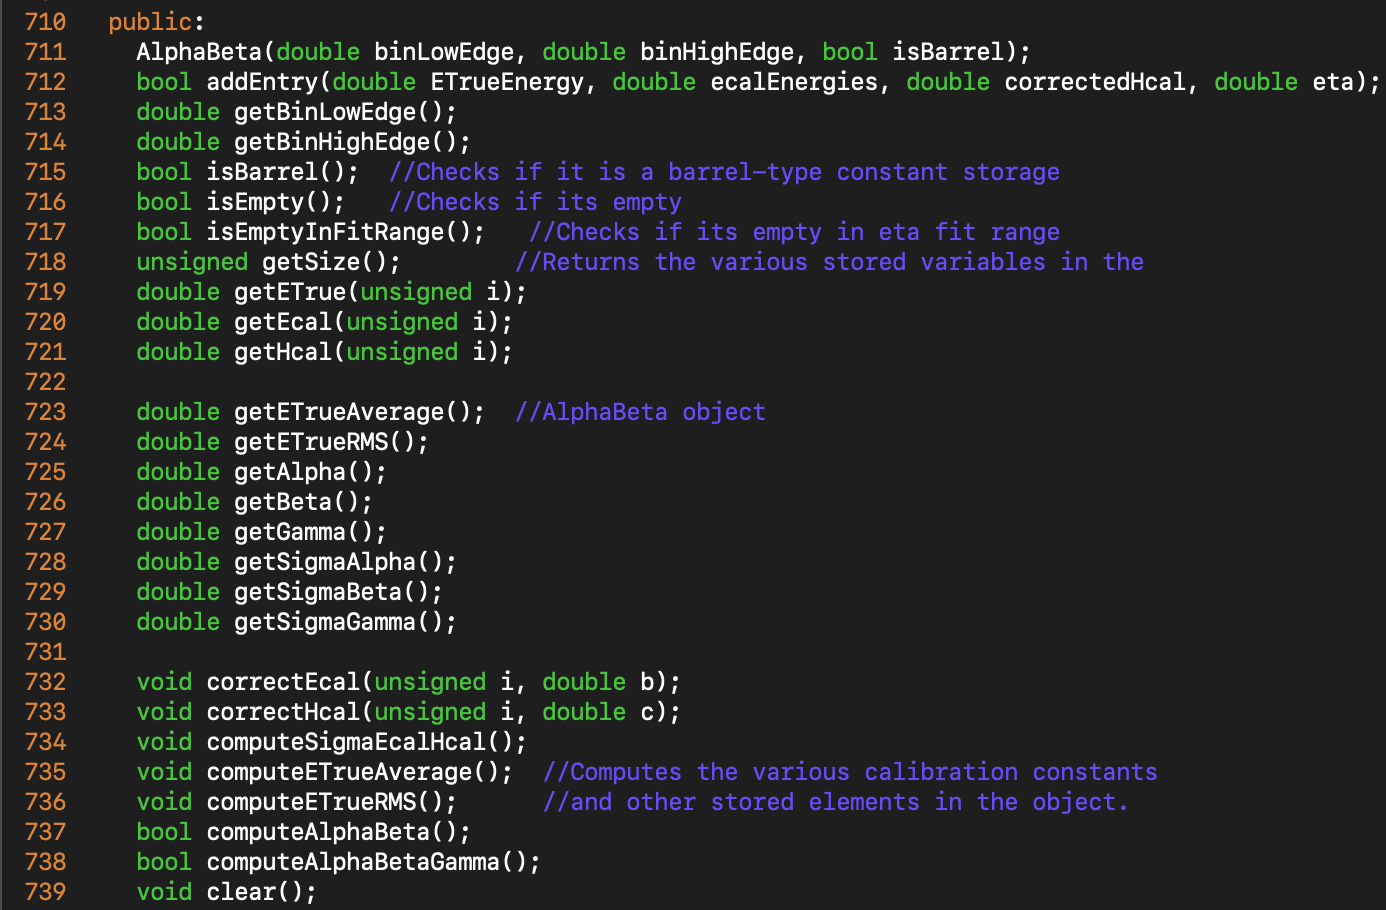
\includegraphics[width=1.0\textwidth]{fig/AlphaBeta.png}
\caption{functions in AlphaBeta class}
\label{AlphaBeta}
%\end{center}
\end{figure}

\subsection{functions}

\subsubsection{InitBarrelAlpha}

It initialize some TF1 type functions. Initialized functions don't use anymore.

\subsubsection {LoadOldThresholds}

Load thereshold values that comes from Shubham who did offline PF hadron calibration. 3.5 is used for EH hadrons and 2.5 is used for H hadrons. Don't foucs on the "old". This value used for Run2 data taking.

\subsubsection {getValuesFromTree}
This function open the ntuples and get value from ntuples. Get generator level information(energy, eta and phi) and get particle flow based information(momentum, id, eta, phi, measured energy in ECAL and HCAL)


\subsubsection {GetETrueBin}


\subsubsection {GetETrueBinEta}


\subsubsection {assignvalues}


\subsubsection {drawCompare}


\subsubsection {drawEtaDependence}


\subsubsection {drawGausFit}



\subsection{classes}

\subsubsection{ABC}

\subsubsubsection{ABC}


\subsubsubsection{addEntry}



\subsubsubsection{getBinLowEdge}



\subsubsubsection{getBinHighEdge}



\subsubsubsection{isBarrel}



\subsubsubsection{isEmpty}



\subsubsubsection{isEmptyInFitRange}



\subsubsubsection{getSize}



\subsubsubsection{getETrueAverage}



\subsubsubsection{getETrueRMS}



\subsubsubsection{getA}



\subsubsubsection{getB}



\subsubsubsection{getC}



\subsubsubsection{getSigmaB}



\subsubsubsection{getSigmaC}



\subsubsubsection{getETrue}



\subsubsubsection{getEcal}



\subsubsubsection{getHcal}



\subsubsubsection{getEta}



\subsubsubsection{getNEntries}



\subsubsubsection{computeETrueAverage}



\subsubsubsection{computeETrueRMS}



\subsubsubsection{computeA}



\subsubsubsection{computeB}



\subsubsubsection{computeC}



\subsubsubsection{computeBC}



\subsubsubsection{clear}


\subsubsection{AlphaBeta}

\subsubsubsection{AlphaBeta}



\subsubsubsection{addEntry}



\subsubsubsection{getBinLowEdge}



\subsubsubsection{getBinHighEdge}



\subsubsubsection{isBarrel}



\subsubsubsection{isEmpty}



\subsubsubsection{isEmptyInFitRange}



\subsubsubsection{getSize}



\subsubsubsection{getETrue}



\subsubsubsection{getEcal}



\subsubsubsection{getHcal}



\subsubsubsection{getETrueAverage}



\subsubsubsection{getETrueRMS}



\subsubsubsection{getAlpha}



\subsubsubsection{getBeta}



\subsubsubsection{getGamma}



\subsubsubsection{getSigmaAlpha}



\subsubsubsection{getSigmaBeta}



\subsubsubsection{getSigmaGamma}



\subsubsubsection{correctEcal}



\subsubsubsection{correctHcal}



\subsubsubsection{computeSigmaEcalHcal}



\subsubsubsection{computeETrueAverage}



\subsubsubsection{computeETrueRMS}



\subsubsubsection{computeAlphaBeta}



\subsubsubsection{computeAlphaBetaGamma}



\subsubsubsection{clear}




\end{document}
